% EXAMPLE: Sections and Paragraphs
% \section		- Level 1
% \subsection		- Level 2
% \subsubsection	- Level 3
% \paragraph		- Level 4
% \subparagraph		- Level 5 
% \section{<NAME_OF_SECTION>}

% EXAMPLE: Include graphics 
% \includegraphics[width=130mm,height=108mm]{intro4.png}

% EXAMPLE: Nested list
%\begin{enumerate}
%\item Nested list
%\begin{enumerate}
%\item
%\item
%\item
%\item
%\item
%\end{enumerate}
%\end{enumerate}

\section{Appendix A - How to build upon our codebase}
This appendix include information on how to build upon our codebase for the Mulle (C), server code (Python, PHP/HTML5 and C) and Android Mobile phone (Java).
\subsection{Mulle}
\subsection{Server}
\subsubsection{Coapy server}
TODO: Python parts such as the python coapy server and how we use EXIP c-code parts. 
\subsubsection{Webpages and database}
\subsection{Android Mobile Phone application}

\subsection{Android}

The primary goals for the android applications were;
%communication goes via a server.
\begin{itemize}
 \item communicate using CoAP over an UDP connection
 \item encode the sent packets with EXI to reduce the size of packets
 \item have a graphical UI capable of controlling multiple devices.
\end{itemize}
% UNDERSÖK OM MER SKA IN HÄR

\subsubsection{The finished product}

The application start off by showing the server menu. One will have to either add a server or use a saved one. 
Clicking on a server in the list will cause the application to validate that the server is alive and thereafter it will perform a CoAP discovery on the server. 
When receiving an answer to the discovery the application will start filling the device menu with devices and their services. The device menu can then be accessed to use the services available.
The services generally works as follows: The application gets a click on the chosen service, so it sends it message to chosen reciever, whereafter the chosen device either changes something or responds.
The device will then have to respond to the application with the updates made, this can be with a confirmation or a whole new CoAP message. This makes the application respond by updating the GUI with the new values.

The pre-built services are generalized to; 
\begin{itemize}
 \item IsOn, provides an item with a checkbox that is checked if a service is on (for example a lamp). Clicking on this should provide a change on the selected device.
 \item GetValue, provides an item which shows the last value provided. Clicking on the item should provide an update.
 \item SendValue, provides an item which have a textbox where one can send a payload to the device. %ska denna även visa vad värdet är för tillfället? tror det 
\end{itemize}

Another planned feature is the options menu where the application will allow things like turning EXI encryption on or off. 

\subsubsection{What exists today}

Today there exists a communication part which allows one to send and recieve CoAP messages. This part uses a library made out of \tttext{jCoAP revision 202b8f8eb7b4, http://code.google.com/p/jcoap/}%s.unger.mobil@gmail.com committer ,	chr.lerche@gmail.com	owner,	nic@nclm.de	owner
to get the CoAP features. This part is not yet a completed project but the features requested for this application is present. The EXI converter is currently not available but is planned to use exificient, 
which can be found at \tttext{http://exificient.sourceforge.net/}.

The GUI is another important part of the application. It is built to be able to controll multiple servers and devices. 
To make this possible the application has 3 tabs:	%the default thought was to have a checkbox in the server menu to allow one to decide whether a server is being currently used, this idea has however been dropped due to lack of time.
\begin{itemize}
 \item Device tab
 \item Server tab
 \item Options tab
\end{itemize}

The Options tab does currently not contain anything but should simply allow a user to change things about how the application should work and what and how things should be displayed. 

 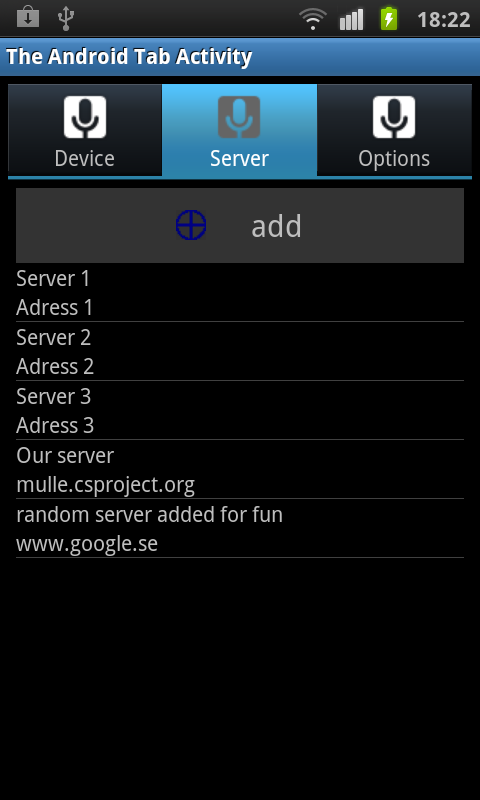
\includegraphics[scale=0.75]{android-server.png}\caption{The Server tab of the Android application}
The Server tab shows all the active servers. You can click on the add button in the server menu and a window appears where you write in the name and adress appear, 
however, the CoAP discovery is not made yet but shouldn't be to far away from completion. The servers then appears in a listview where it's easy to keep track of them.
In the future this can be complemented with a network discovery of nodes, however, my personal opinion is that it should be possible to manually add an server.

 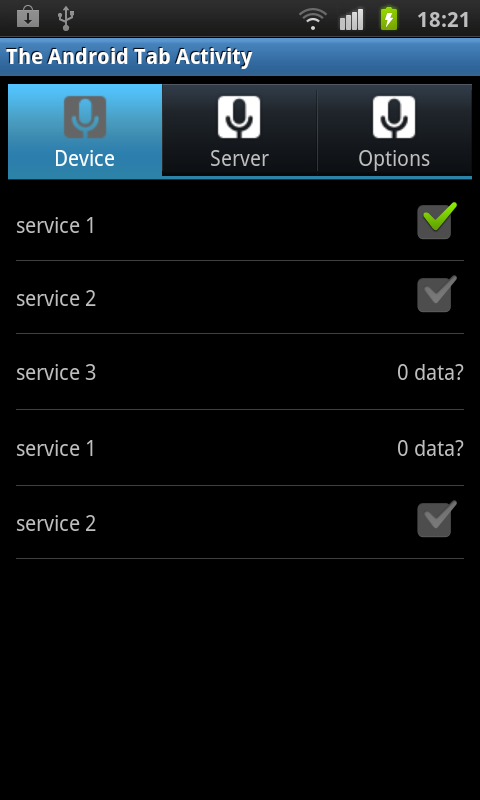
\includegraphics[scale=0.75]{android-device.png}\caption{The device tab of the Android application}
The Device tab is the latest addition in the GUI and contains the actual services that are available. It contains a custom listadapter that have been tweaked to be able to display children of the interface rowdata.
In it's current state it is possible to add items to this list in the code by calling the NewItem() function with proper parameters. Adding service types if the pre-built service types are not enough is easy. 
Simply extend the rowdata() interface and create the desired xml for the item, do not however forget to add a typenumber for the NewItem() function to be able to create it. 
It also allows the children to define for their own what should happen if clicked, updated and so on.






